\documentclass{article}
% NeurIPS 2025 style (neurips_2025.sty, in this folder) as a preprint: author names shown, no line numbers.
\usepackage[preprint,nonatbib]{neurips_2025}
\usepackage[utf8]{inputenc}
\usepackage[T1]{fontenc}
\usepackage{amsmath,amssymb}
\usepackage{booktabs}
\usepackage{graphicx}
\usepackage{xcolor}
\usepackage{microtype}
\usepackage[numbers,sort&compress]{natbib}
\usepackage{hyperref}
\hypersetup{colorlinks=true,linkcolor=blue!50!black,citecolor=blue!50!black,urlcolor=blue!50!black}
% Generated by paper_bridges/make_assets.py from results/multiagent/: do not edit.
\newif\ifCOneD\COneDfalse
\newcommand{\BThreeFittedCalled}{5}
\newcommand{\BThreeFittedRight}{4}
\newcommand{\BThreeNaiveCalled}{6}
\newcommand{\BThreeNaiveRight}{3}
\newcommand{\BThreeUnfittedCalled}{6}
\newcommand{\BThreeUnfittedRight}{2}
\newcommand{\BridgeGain}{+0.013}
\newcommand{\BridgeGainCI}{[-0.002, 0.027]}
\newcommand{\BridgeGainP}{0.062}
\newcommand{\CArrivalRole}{88}
\newcommand{\CCrossOne}{0.023}
\newcommand{\CCrossRole}{0.126}
\newcommand{\CRelayOne}{0.9}
\newcommand{\CRelayRole}{24.3}
\newcommand{\CleanBridgeOne}{-0.058}
\newcommand{\CleanBridgeOneCI}{[-0.064, -0.051]}
\newcommand{\CleanBridgeOneP}{0.031}
\newcommand{\CleanCoupled}{-0.092}
\newcommand{\CleanCoupledCI}{[-0.102, -0.085]}
\newcommand{\CleanCoupledP}{0.031}
\newcommand{\ContamBridgeOneB}{0.334}
\newcommand{\ContamWindowB}{0.375}
\newcommand{\CostB}{24.18}
\newcommand{\CostC}{10.57}
\newcommand{\CostOne}{26.01}
\newcommand{\CouplingCost}{0.092}
\newcommand{\CouplingCostCI}{[0.081, 0.103]}
\newcommand{\CouplingCostP}{0.031}
\newcommand{\CrossBridgeGuard}{0.193}
\newcommand{\CrossBridgeOne}{0.006}
\newcommand{\EvidenceEffect}{-0.001}
\newcommand{\EvidenceEffectCI}{[-0.005, 0.004]}
\newcommand{\EvidenceEffectP}{0.688}
\newcommand{\FilterGain}{-0.027}
\newcommand{\FilterGainCI}{[-0.052, -0.001]}
\newcommand{\FilterGainP}{0.953}
\newcommand{\FixMinusWindow}{-0.002}
\newcommand{\FixMinusWindowCI}{[-0.008, 0.005]}
\newcommand{\FixMinusWindowP}{0.719}
\newcommand{\GateBI}{-0.003}
\newcommand{\GateBICI}{[-0.022, 0.014]}
\newcommand{\GateBII}{-0.048}
\newcommand{\GateBIICI}{[-0.096, 0.002]}
\newcommand{\GateBIIP}{0.059}
\newcommand{\GateBIIUpper}{-0.006}
\newcommand{\GateBIP}{0.617}
\newcommand{\GateCI}{-0.013}
\newcommand{\GateCICI}{[-0.029, 0.002]}
\newcommand{\GateCII}{-0.040}
\newcommand{\GateCIICI}{[-0.079, -0.004]}
\newcommand{\GateCIIP}{0.059}
\newcommand{\GateCIIUpper}{-0.010}
\newcommand{\GateCIP}{0.918}
\newcommand{\GateCIWelfare}{-0.018}
\newcommand{\GateCIWelfareCI}{[-0.040, 0.002]}
\newcommand{\GateCIWelfareP}{0.922}
\newcommand{\GateOneBar}{0.085}
\newcommand{\GateOneI}{+0.105}
\newcommand{\GateOneICI}{[0.086, 0.125]}
\newcommand{\GateOneII}{+0.020}
\newcommand{\GateOneIICI}{[0.001, 0.037]}
\newcommand{\GateOneIIP}{0.047}
\newcommand{\GateOneIP}{0.004}
\newcommand{\GateOneIWelfare}{+0.136}
\newcommand{\GateOneIWelfareCI}{[0.112, 0.160]}
\newcommand{\GateOneIWelfareP}{0.004}
\newcommand{\GateOneLead}{+0.171}
\newcommand{\GateOneLeadCI}{[0.156, 0.186]}
\newcommand{\GateOneLeadP}{0.004}
\newcommand{\GuardBridgeFalseRelay}{0.212}
\newcommand{\GuardBridgeFalseRelayCI}{[0.015, 0.568]}
\newcommand{\GuardBridgeFalseRelayP}{0.125}
\newcommand{\GuardBridgePooled}{-0.005}
\newcommand{\GuardBridgePooledCI}{[-0.012, 0.006]}
\newcommand{\GuardBridgePooledP}{0.844}
\newcommand{\Interaction}{-0.009}
\newcommand{\InteractionCI}{[-0.016, -0.002]}
\newcommand{\InteractionP}{0.938}
\newcommand{\PooledBridgeOne}{0.183}
\newcommand{\PooledCoupled}{0.159}
\newcommand{\PooledOneBoard}{0.077}
\newcommand{\PooledSquads}{0.248}
\newcommand{\RelayRateBridgeFix}{7.1}
\newcommand{\RelayRateBridgeRole}{21.9}
\newcommand{\RelayRateOne}{0.5}
\newcommand{\RelayRateRelayEvid}{0.5}
\newcommand{\RoleEffect}{+0.016}
\newcommand{\RoleEffectCI}{[0.010, 0.023]}
\newcommand{\RoleEffectP}{0.031}
\newcommand{\SecondBridge}{+0.014}
\newcommand{\SecondBridgeCI}{[-0.006, 0.035]}
\newcommand{\SecondBridgeP}{0.188}
\newcommand{\WinBack}{14}
\newcommand{\WinBackCI}{[-2, 32]}
\newcommand{\WinBackFix}{30}

\newcommand{\pending}[1]{\textcolor{orange!70!black}{[#1]}}

\title{Bridges Between Squads: Moving Information Across Team Boundaries Without Moving the Lies}

\author{%
  Chuntao Dan \\
  \And
  Claude Opus 5.5\thanks{An AI model made by Anthropic, working as a research and coding agent in Claude Code; see the author contributions.} \\
  Anthropic \\
}

\begin{document}
\maketitle

\begin{abstract}
Splitting a large team of language-model agents into squads, each with its own shared board and its own guards, keeps the team effective and safe as it grows, but only while each squad's work stays inside the squad. We give 64 Claude Haiku 5.5 agents, a quarter of them scripted liars, subtasks whose clues span two squads, and test ways to move information across the border under analysis plans frozen before each run. Coupling costs squads $\CouplingCost$ in honest agents' pooled share. One bridge agent per pair of squads beats one shared board of 64 ($\GateOneI$, $p = \GateOneIP$) but wins back only $\WinBack$\% of the coupling cost, because it relays on $\RelayRateOne$\% of its turns. Making relays checkable did not help; a dedicated bridge relayed far more and was safer, but on fresh seeds it was no more effective than the plain bridge ($\GateCI$, $p = \GateCIP$): the busier courier also carried more lies between squads. An exploratory five-board edge did not replicate, and both forecasts recorded before the confirmation called its gate a pass.
\ifCOneD
A window that shows each squad the other squad's posts on shared clues, with no bridge agent, \GateDVerdict{} its confirmation on fresh seeds ($\GateDI$, $p = \GateDIP$).
\else
\pending{A confirmation of a bridge-free design, a window that shows each squad the other squad's posts on shared clues, is running; its result goes here.}
\fi
\end{abstract}

\section{Introduction}

Teams of language-model agents grow by adding members, and a shared space where every member posts and reads is the simplest way to pool what they know. Our earlier work found that on such a board a few scripted liars take most of what honest agents earn, that guards (agents assigned to check and contest posted values, never to solve) recover much of that damage, and that the guards' advantage fades as one board grows to 64 agents because they hold too few of the clues; squads of eight, each with its own board, subtasks and guards, kept it (Dan and Claude, companion preprint). Squads raise the obvious next question. Real work rarely splits cleanly, and squads that never exchange information leave value on the table. This paper asks how to move information across squad borders without also moving the lies.

We find four things.
\begin{enumerate}
\item \textbf{Coupling costs squads, and one bridge wins little of it back} (\S\ref{sec:c1}). When a quarter of each squad's subtasks need a clue held in the next squad, honest pooled share falls by $\CouplingCost$ $\CouplingCostCI$. One bridge agent per pair of squads still beats one shared board of 64, but recovers only $\WinBack$\% of the coupling cost: it relays on $\RelayRateOne$\% of its turns.
\item \textbf{Making relays checkable does not make bridges relay; making the bridge a role does, but more relays are not more value} (\S\ref{sec:c1b}). Evidence on relayed values changed nothing ($\EvidenceEffect$); a dedicated bridge raised honest pooled share by $\RoleEffect$ over five exploratory boards and cut contamination.
\item \textbf{The dedicated bridge did not replicate} (\S\ref{sec:confirm}). On eight fresh seeds it relayed on $\CRelayRole$\% of its turns (the plain bridge $\CRelayOne$\%) and was safer, but honest pooled share moved by $\GateCI$ $\GateCICI$: it also carried more lies between squads (cross-squad contamination $\CCrossRole$ against $\CCrossOne$).
\item \textbf{Small exploratory screens mislead, and so do forecasts built on them} (\S\ref{sec:forecasts}). Both lines of forecasts recorded before the confirmation called its gate wrong.
\end{enumerate}
\ifCOneD
\else
\pending{C1d, a window onto the other squad's posts with no bridge agent, is the last confirmation in this series; the abstract, \S\ref{sec:confirm} and the discussion are completed when it has run.}
\fi

\section{Related work}

Moving information between groups has a long history in organizational research, where boundary-spanning individuals carry it between an organization's units \citep{tushman1981boundary}. For language-model agents, orchestrator-and-worker systems pass information through one coordinator \citep{anthropic2025research}, and across many configurations multi-agent architectures range from large gains to large losses against a single agent \citep{kim2025scaling}. Groups of language models also pool too little of what their members know \citep{li2026hiddenbench,anthropic2026redteam}, the problem squads trade off against containment. Defences against faulty members include credibility scores, inspector roles and agreement counts \citep{ebrahimi2025credibility,huang2024faulty,seeley2010honeybee}. What we add is a controlled test, under frozen plans and on fresh seeds, of how information should cross a squad border when some members lie.

\section{Methods}

\paragraph{The clue board and squads.} Each subtask is a hidden residue; its clues are dealt to two agents each, so an honest holder can contradict a lie about it. Agents post clue values to their squad's board, which counts how many agents posted each value (confirmed at two, contested when values disagree), and answer subtasks; a correct answer scores, a wrong one costs. 64 Claude Haiku 5.5 agents form eight squads of eight, each with its own board, subtasks and two guards, 40 turns, full memory. A quarter of the agents are scripted liars that post false values for clues of subtasks they do not work on; the measure is the honest agents' pooled share of the welfare available (\emph{honest pooled share}), with raw honest welfare as a robustness check. \emph{Contamination} is the share of answers built on a false value.

\paragraph{Coupling, mirrors and bridges.} In a coupled world every fourth subtask of a squad needs one clue held only in the next squad. That clue appears on the next squad's board as a \emph{mirror} line: its holders can post a value there but cannot answer, and that squad's liars lie there too. Arms (Table~\ref{tab:arms}) differ only in how a mirror value reaches the squad that needs it.

\begin{table}[t]
\centering\small
\caption{Arms. All at 64 agents in squads of 8 with two guards each; scripted liars in a quarter of the slots, or none on clean boards.}
\label{tab:arms}
\begin{tabular}{@{}lp{7.6cm}l@{}}
\toprule
Arm & What crosses the border & Experiment \\
\midrule
squads, uncoupled & nothing needs to & C1 (reference) \\
coupled & nothing can & C1 \\
one bridge & one honest solver per squad pair reads the neighbour's mirrors and may relay a value & C1 \\
two bridges; guard bridge & two such solvers; a guard as the bridge & C1 \\
evidence & as one bridge, and a relayed value shows its mirror tally & C1b \\
role (dedicated bridge) & the bridge relays and never solves & C1b, C1c \\
both & evidence and the dedicated bridge & C1b \\
mirror window & no bridge; every coupled clue's mirror tally shows from the start & C1b, C1d \\
\bottomrule
\end{tabular}
\end{table}

\paragraph{Design and statistics.} Each experiment's plan (arms, seeds, gate, secondary tests and hand-recorded forecasts) was frozen, hashed and pushed before its run. Arms are paired on board seed; tests are exact one-sided sign-flip tests over seeds (8 seeds give a smallest $p$ of 1/256, 5 seeds 1/32), with bootstrap intervals over seeds. A safety part is a non-inferiority test: the 95th percentile of 2,000 paired bootstrap means of the contamination difference must lie below a margin of 0.05. C1 and C1b used seeds 1800--1807; the confirmations used fresh seeds (C1c 1810--1817, C1d 1820--1827). Every reply is cached, so every reported number can be rebuilt from the saved runs at no cost.

\section{Results}

\begin{figure}[t]
\centering
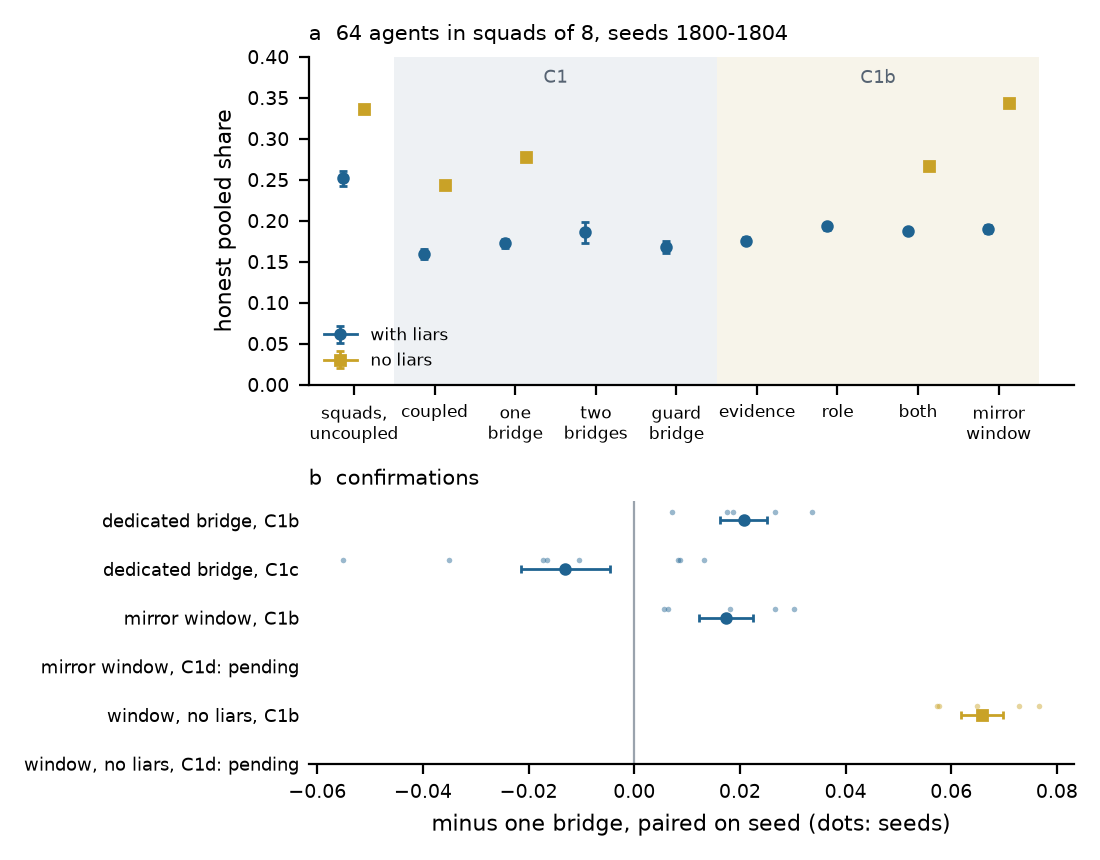
\includegraphics[width=\linewidth]{figures/bridges.png}
\caption{\textbf{a}, honest pooled share per arm on seeds 1800--1804 (mean $\pm$ SEM over boards), with liars (circles) and on clean boards (squares, where run). \emph{evidence}: relays show their mirror tally; \emph{role}: a dedicated bridge; \emph{both}: the two together. \textbf{b}, each design minus one bridge, paired on seed: the exploratory boards of C1b (5 seeds) against the confirmations on fresh seeds (8 seeds); small dots are seeds. * $p < 0.05$, two-sided exact sign-flip test against 0 (five seeds cannot reach it).}
\label{fig:bridges}
\end{figure}

\subsection{Coupling costs squads; one bridge wins little back (C1)}
\label{sec:c1}

One bridge per pair of squads beat one shared board of 64 agents by $\GateOneI$ $\GateOneICI$ in honest pooled share ($p = \GateOneIP$, 8 boards) and kept at least half of the uncoupled squads' lead (margin $\GateOneII$, $p = \GateOneIIP$; the lead $\GateOneLead$), robust on raw welfare ($\GateOneIWelfare$). By that gate, squads with bridges are worth training in. But the bridge did little. Against coupled squads with no bridge it added $\BridgeGain$ $\BridgeGainCI$, $\WinBack$\% of the $\CouplingCost$ that coupling costs ($\WinBackCI$\%), because it relayed on $\RelayRateOne$\% of its turns. A second bridge added $\SecondBridge$; a guard as the bridge lowered the share of false relays by $\GuardBridgeFalseRelay$ without changing honest pooled share ($\GuardBridgePooled$). Without liars, coupled squads scored $\CleanCoupled$ against uncoupled ones, and with one bridge $\CleanBridgeOne$ (Figure~\ref{fig:bridges}a).

\subsection{Evidence does not make bridges relay; a role does (C1b)}
\label{sec:c1b}

Two fixes targeted the bridge's silence. \emph{Evidence} shows the receiving squad a relayed value's mirror tally, so a relay can be checked; the \emph{dedicated bridge} relays and never solves. Their combination was no more effective than one bridge ($\GateBI$ $\GateBICI$, $p = \GateBIP$) but was safer (contamination $\GateBII$, 95th percentile $\GateBIIUpper$), so its gate asked us to decide. In the exploratory $2\times 2$ (5 boards), the role raised honest pooled share by $\RoleEffect$ $\RoleEffectCI$ and evidence did nothing ($\EvidenceEffect$); bridges relayed on $\RelayRateRelayEvid$\% of turns with evidence alone, $\RelayRateBridgeRole$\% as dedicated bridges. Evidence also did not filter lies at the border (filter gain $\FilterGain$). A window that showed every coupled clue's mirror tally from the start, with no bridge, did as well as the combination with liars ($\FixMinusWindow$ for the combination minus the window) and on clean boards was level with uncoupled squads.

\subsection{Confirmations on fresh seeds}
\label{sec:confirm}

The dedicated bridge was the best coupled arm on C1b's five boards (above one bridge on all five), but it was chosen after seeing them. On eight fresh seeds (C1c) it was not more effective: $\GateCI$ $\GateCICI$, $p = \GateCIP$ (raw welfare $\GateCIWelfare$). It was safer (contamination $\GateCII$, 95th percentile $\GateCIIUpper$) and it did relay: on $\CRelayRole$\% of its turns against $\CRelayOne$\%, with $\CArrivalRole$\% of relays confirmed on arrival. But it also carried more lies between squads: cross-squad contamination $\CCrossRole$ against $\CCrossOne$. The value of the extra relays and the harm of the relayed lies roughly cancelled (Figure~\ref{fig:bridges}b).

\ifCOneD
The mirror window, the other design that led on C1b's five boards, was confirmed on eight more fresh seeds (C1d): with liars $\GateDI$ $\GateDICI$, $p = \GateDIP$ (raw welfare $\GateDIWelfare$), contamination $\GateDII$ (95th percentile $\GateDIIUpper$); its gate \GateDVerdict. On clean boards it differed from one bridge by $\DClean$ $\DCleanCI$ ($p = \DCleanP$, \DCleanSupported).
\else
\pending{C1d: the mirror window against one bridge on seeds 1820--1827, with liars (the gate) and clean (a secondary test).}
\fi

\subsection{Forecasts before the runs}
\label{sec:forecasts}

Each plan recorded forecasts before its run. For C1, a simulator of rule agents fitted to earlier Claude runs called $\BThreeFittedRight$ of $\BThreeFittedCalled$ effect directions right, against $\BThreeUnfittedRight$ of $\BThreeUnfittedCalled$ unfitted and $\BThreeNaiveRight$ of $\BThreeNaiveCalled$ for a naive rule. For C1c, both hand-recorded lines, one reading only C1b's five boards and one assuming every design helps, called the gate a pass; it failed. Five paired boards that agree in sign are weak evidence when the effect is about 0.02 in honest pooled share and the arm was picked because it led.

\section{Discussion}

Squads contain lies by containing information; any channel that lets information cross a squad border is also a channel for lies. A bridge that rarely relays is safe and nearly useless, and a bridge that relays often is useful and leaky, so that in our runs the two cancelled. Checkable relays did not change this, because the bridge's silence, not the receiver's trust, was the bottleneck. For training (our next step is reinforcement learning of a 3B open model in this world), the choice of channel sets what agents can learn: we keep the border contest credit, which pays a holder whose post on a mirror line contests a false value.
\ifCOneD\else\ \pending{The training world's channel follows C1d.}\fi

\paragraph{Limitations.} One model (Claude Haiku 5.5), one task family and scripted liars; one squad size (8) and one coupling rate (a quarter of subtasks); five-board secondary contrasts, uncorrected and exploratory; the window was the one design chosen after seeing C1b, and was confirmed for that reason.

\paragraph{Author contributions.} C.D. set the questions and the design decisions and approved every plan and cost. Claude Opus 5.5 wrote the code, plans, analyses and text under C.D.'s direction.

\bibliographystyle{abbrvnat}
\bibliography{references}

\appendix
\section{Plans, costs and reproduction}
\label{app:repro}

Plans: C1 \texttt{specs/multiagent/phase20/}, C1b \texttt{phase23/}, C1c \texttt{phase24/}, C1d \texttt{phase25/}, each frozen and hashed before its run. API cost: C1 \$\CostOne, C1b \$\CostB, C1c \$\CostC\ifCOneD, C1d \$\CostD\fi{} (pilots included). Every number in this paper is a macro written by \texttt{paper\_bridges/make\_assets.py} from the saved results.

\end{document}
